\documentclass[a4paper,10pt]{article}
\usepackage[T1]{fontenc}
\usepackage[utf8]{inputenc}
\usepackage{lmodern}
\usepackage{url,csquotes}
\usepackage{fancyhdr}
\usepackage{graphicx}
\usepackage{epstopdf}
\usepackage{lastpage}
\usepackage{listings}
\usepackage{fancyref}
%\usepackage{subfigure}
\usepackage{enumitem}
\usepackage{tabularx, booktabs ,multirow}
\usepackage{mathtools}
\usepackage{caption}
\usepackage{subcaption}
\captionsetup{justification=centering}
\usepackage{anysize} %%pour pouvoir mettre les marges qu'on veut 
\marginsize{2cm}{2cm}{2cm}{2cm} 

\usepackage{amsfonts,amssymb,amsmath,amsthm} 
\newcommand{\vect}[2]{ $\begin{pmatrix} #1 \\  #2 \end{pmatrix} $  }

\newcommand{\matrice}[3]{ \begin{pmatrix}  #1 &  #3 \\ #3  & #2 \end{pmatrix}   }

\newcommand{\norm}[1]{\left\lVert #1 \right\rVert} 
\newcommand{\norme}[1]{\left\lVert #1 \right\rVert_2} 
\newcommand{\fsurg}{\frac{f}{g}} 
\newcommand{\prodv}[2]{ #1^T #2 } 

\usepackage{enumitem} 

% Graph package
\usepackage{tikz}
\usetikzlibrary{arrows}

\begin{document}


\begin{center}
\rule{\textwidth}{3pt}
Master MVA \\
Dynamic Programming \& Reinforcement Learning \\
TP2 - 27/11/2016 \\
\textsc{ Achari Berrada Youssef} \\
\rule{\textwidth}{.3pt}
\end{center}

\section{Q-Learning :}
\begin{enumerate}[label=\underline{\textbf{Q\arabic*}:}]
\item The exploration policy is the $\epsilon$-greedy policy. I choose $\epsilon = 0.4$ so that we explore all the action-states.
With probability $1 - \epsilon$, we choose $ a_t = \text{argmax} \, Q(x_t,a)$, and with probability $\epsilon$, we choose a random action. This exploration policy allows us to explore a large set of state-actions in order to satisfy the stochastic approximation requirement. I choose the learning rate to be : 

\[ \alpha(x,a) = \frac{1}{N(x,a)}\]

Performance evolution over $T = 1000$ episodes: 

\begin{figure}[!h]
\centering
 		\begin{subfigure}[b]{0.5\textwidth}
                \centering
                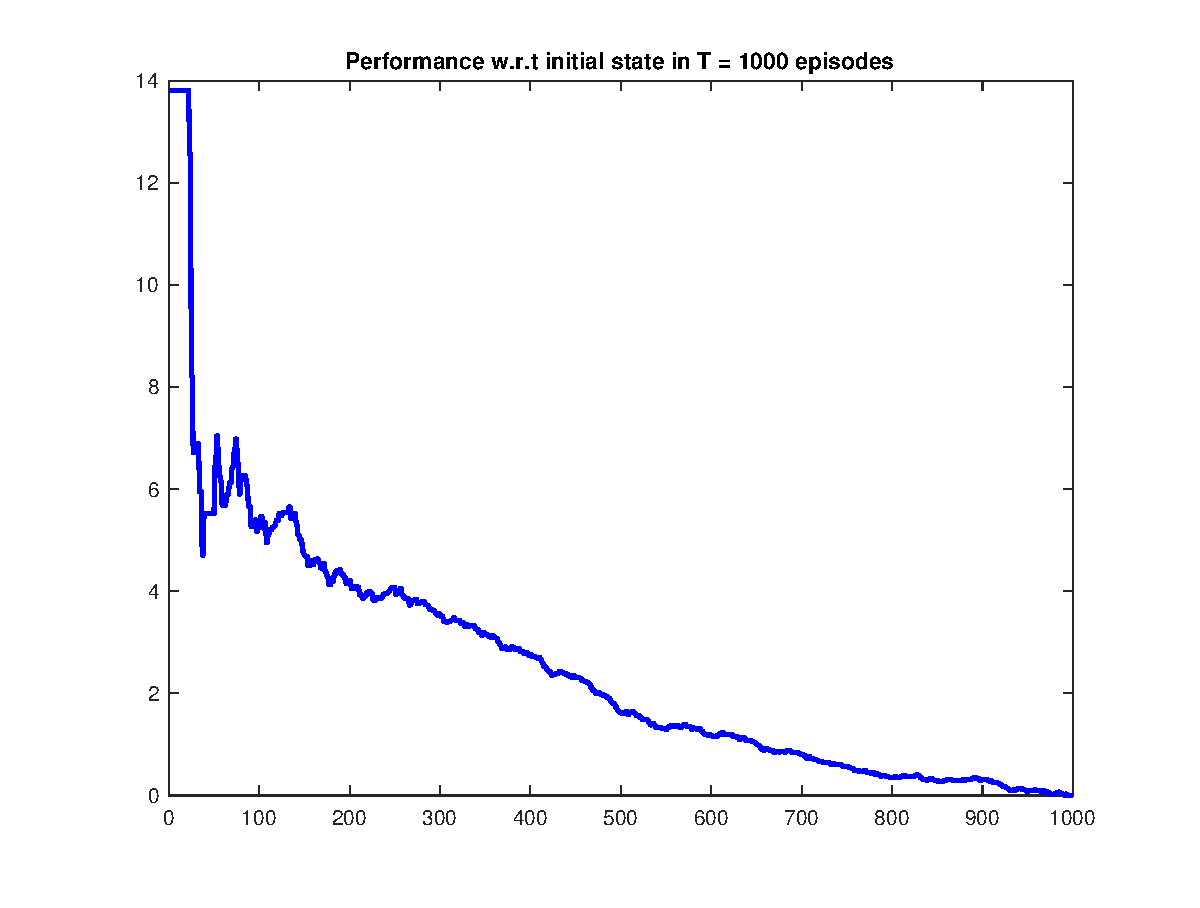
\includegraphics[width=.95\linewidth]{Figure/QLearnInit.eps}  
                \caption{Performance in state 1.}
                \label{fig:sameL}
        \end{subfigure}%
        \begin{subfigure}[b]{0.5\textwidth}
                \centering
                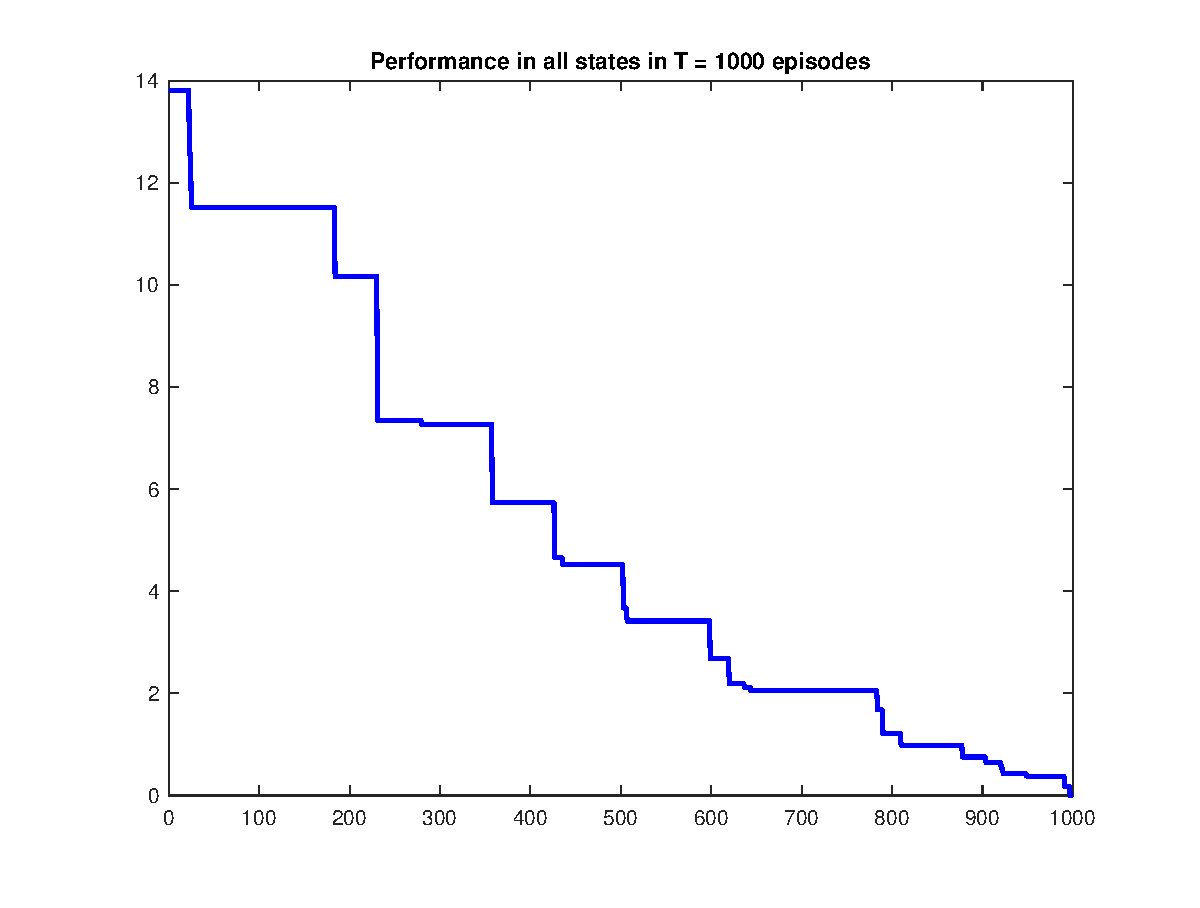
\includegraphics[width=.95\linewidth]{Figure/QLearnAll.eps}  
                \caption{Error Propagation. }
                \label{fig:errorP}
        \end{subfigure}
\caption{Performance of the Q-Learning algorithm.}%\label{fig:animals}
\end{figure}

\section{Stochastic Multi-Armed Bandits on simulated Data} 
\item

\end{enumerate}

\end{document}
